%! TEX root = main.tex
\documentclass[12pt, a4paper]{article}

\usepackage{graphicx} % Required for inserting images
\usepackage[utf8]{inputenc}
\usepackage[english, russian]{babel}
\usepackage{times}
\usepackage{fontspec} 
\usepackage{titlesec}
\usepackage{amsmath}
\usepackage[normalem]{ulem}
\usepackage[htt]{hyphenat}
\usepackage{amssymb}
\usepackage{mathtools}
\usepackage{wrapfig}
\usepackage{tabularx}
\usepackage{svg}
\usepackage{subcaption}
\usepackage{pdfpages}
\renewcommand{\thesubfigure}{\asbuk{subfigure}} % а, б, в...
\usepackage[normalem]{ulem}
\numberwithin{equation}{section}
\defaultfontfeatures{Ligatures={TeX},Renderer=Basic} 
\usepackage{appendix}
\setmainfont[Ligatures={TeX,Historic}]{Times New Roman}

% \usepackage{polyglossia}
% \setmainlanguage[Script=Cyrillic]{russian}

\usepackage{biblatex}
\addbibresource{sources.bib}

\usepackage{indentfirst}
\setlength\parindent{12.5mm}

\usepackage{geometry}
% \geometry{
%     a4paper,
%     left=30mm,
%     right=10mm,
%     top=20mm,
%     bottom=20mm
% }
\geometry{
  a4paper,
  top=2cm,
  bottom=2cm,
  left=2.5cm,
  right=1cm
} %, heightrounded, showframe

\usepackage{array,supertabular,hhline,enumitem,hyperref}
\usepackage{listings}
\usepackage{xcolor}
\usepackage{longfbox,fancyhdr}
\definecolor{codegreen}{rgb}{0,0.6,0}
\definecolor{codegray}{rgb}{0.5,0.5,0.5}
\definecolor{codepurple}{rgb}{0.58,0,0.82}

\lstset{
    backgroundcolor=\color{white},
    commentstyle=\color{codegreen},
    keywordstyle=\color{magenta},
    numberstyle=\tiny\color{codegray},
    stringstyle=\color{codepurple},
    basicstyle=\ttfamily\footnotesize,
    breakatwhitespace=false,
    breaklines=true,
    captionpos=t,
    keepspaces=true,
    numbers=left,
    numbersep=5pt,
    showspaces=false,
    showstringspaces=false,
    showtabs=false,
    tabsize=2,
    frame=single,
}

\lstset{
    rangeprefix=\#\ SECTION\ ,
    % rangebeginprefix=\#\ SECTION,
    % rangeendprefix=#\ SECTION,
    rangebeginsuffix=\ BEGIN,
    rangeendsuffix=\ END,
    includerangemarker=false
}

\newcommand\listingsection[2]{
  \lstinputlisting[
    language=python,
    linerange=#2-#2
  ]{#1}
}

\let\stdsection\section
\renewcommand\section{\clearpage\stdsection}

\usepackage{setspace}
\onehalfspacing


%%% Основные сведения %%%
\newcommand{\thesisAuthorLastName}{Скоробогатов}
\newcommand{\thesisAuthorOtherNames}{Егор Викторович}
\newcommand{\thesisAuthorInitials}{Е. В.}
\newcommand{\thesisAuthor}             % Диссертация, ФИО автора
{%
    \texorpdfstring{% \texorpdfstring takes two arguments and uses the first for (La)TeX and the second for pdf
        \thesisAuthorLastName~\thesisAuthorOtherNames% так будет отображаться на титульном листе или в тексте, где будет использоваться переменная
    }{%
        \thesisAuthorLastName, \thesisAuthorOtherNames% эта запись для свойств pdf-файла. В таком виде, если pdf будет обработан программами для сбора библиографических сведений, будет правильно представлена фамилия.
    }
}
\newcommand{\thesisAuthorShort}        % Диссертация, ФИО автора инициалами
{\thesisAuthorInitials~\thesisAuthorLastName}
%\newcommand{\thesisUdk}                % Диссертация, УДК
%{\fixme{xxx.xxx}}
\newcommand{\thesisTitle}              % Диссертация, название
{Визуальная система телеоперации манипулятором с двухпальцевым захватом}
\newcommand{\thesisSpecialtyNumber}    % Диссертация, специальность, номер
{15.03.06}
\newcommand{\thesisSpecialtyTitle}     % Диссертация, специальность, название (название взято с сайта ВАК для примера)
{Мехатроника и робототехника}
\newcommand{\thesisDegree}             % Диссертация, ученая степень
{бакалавра}
\newcommand{\thesisDegreeShort}        % Диссертация, ученая степень, краткая запись
{бак.}
\newcommand{\thesisCity}               % Диссертация, город написания диссертации
{Москва}
\newcommand{\thesisYear}               % Диссертация, год написания диссертации
{\the\year}
\newcommand{\thesisOrganization}       % Диссертация, организация
{
  Федеральное Государственное Бюджетное
  Образовательное Учреждение Высшего Образования <<Национальный
  Исследовательский Университет <<МЭИ>>
}


\newcommand{\supervisorFio}              % Научный руководитель, ФИО
{Адамов Борис Игоревич}
\newcommand{\supervisorRegalia}          % Научный руководитель, регалии
{доц.}
\newcommand{\supervisorFioShort}         % Научный руководитель, ФИО
{Б. И. Адамов}
\newcommand{\supervisorRegaliaShort}     % Научный руководитель, регалии
{доц.}

\newcommand{\wideunderline}[2][2em]{%
  \underline{\makebox[\ifdim\width>#1\width\else#1\fi]{#2}}%
}


\begin{document}
\onehalfspacing

% \begin{wrapfigure}{L}{\textwidth}
%   
\includegraphics[width=0.156\textwidth]{images/mpei_logo.jpg}
% \end{wrapfigure}
\begin{center}

\textbf{МИНОБРНАУКИ РОСИИ}\\
федеральное государственное бюджетное образовательное
учреждение высшего образования
\textbf{<<Национальный исследовательский университет <<МЭИ>>}
\end{center}
\hrule 

\hfill

\textbf{Институт} \hfill \wideunderline[6em]{ЭнМИ} \par
\textbf{Кафедра} \hfill \wideunderline[6em]{РМДиПМ}\par
\begin{center}
\large\textbf{
ЗАДАНИЕ
НА ВЫПУСКНУЮ КВАЛИФИКАЦИОННУЮ РАБОТУ
(БАКАЛАВРСКУЮ РАБОТУ)
}
\end{center}

\uline{\textbf{Направление} \hfill \thesisSpecialtyNumber \
\thesisSpecialtyTitle}\par

\uline{
  \textbf{Образовательная программа} 
  Компьютерные технологии управления
  в робототехнике и мехатронике
}\par

\uline{\textbf{Форма обучения} \hfill очная}\par

\uline{\textbf{Тема:} \hfill \thesisTitle}


\uline{Студент \hfill С-12а-21 \hfill \thesisAuthorLastName \
\thesisAuthorInitials \par}

\par

\uline{
  Руководитель ВКР \hfill к.ф.-м.н. \hfill доцент \hfill \qquad \hfill Адамов Б. И.
}\par

\newpage


\section{Введение}
С развитием машинного обучения и его применения в робототехнике, выросла
нужда в записи данных для обучения так называемых "embodied AI". Также
очень полезной практикой является запись данных в реальных и разных
условиях.

В данной работе представлена система для определения трехмерного
положения кисти в пространстве с использованием двух камер. Эта система
может использоваться для записи датасетов для обучения роботов построению
траекторий, управлению мехатронными телами, а также для простого
запоминания повторяемых действий. Система включает в себя модули
калибровки камер, распознавания рук и триангуляции, что позволяет точно
определять координаты ключевых точек рук в реальном времени.

\section{Постановка задачи}
В своей работе я буду создавать систему для определения положения руки в
трехмерном пространстве и приведения ее к виду двухпальцевого захвата
манипулятора.
Блок-схема задачи изображена на рисунке ~\ref{fig:problem_block_scheme}. 
\begin{figure}[h!]
  \begin{center}
    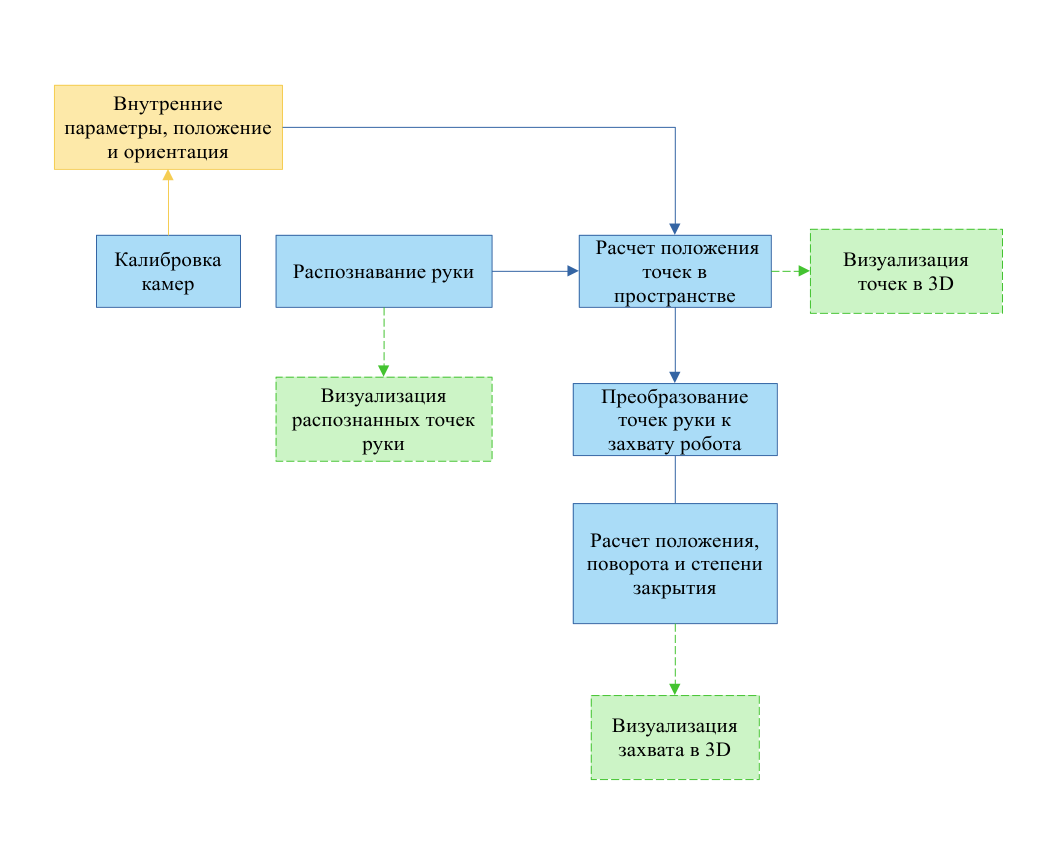
\includegraphics[width=0.95\textwidth]{images/block-schemes/problem_scheme.png}
  \end{center}
  \caption{
    Блок-схема поставленной задачи. Синим обозначены основные
    исполняемые модули, зеленым --- вспомогательные модули, а жёлтым ---
    данные.
  }
\label{fig:problem_block_scheme}
\end{figure}

\subsection{Калибровка камер}
Как далее будет сказано, у камер есть ряд параметров, которые необходимы для
корректного расчета координат в трехмерном пространстве. Некоторые из этих
параметров, такие как положение и поворот могут меняться, однако другие
параметры, о которых сказано в разеделе \ref{sec:camera_model} являются
постоянными.  Система, которую я пишу в рамках этой работы должна быть способна
найти эти параметры, то есть откалибровать камеру.
\par
Также для корректного определения положения точки в пространстве относительно
камеры, нужно знать положение камер относительно заданной точки отсчета системы
координат. То есть система также должна будет определить положение камер
относительно как либо отмеченного начала координат.

\subsection{Получение изображений и их обработка}
Система, создаваемая в этой работе должна:
\begin{itemize}
    \item Принимать на вход либо устройство ввода, то есть камеру или видео,
    \item открывать это видео для захвата изображений,
    \item проводить какую-то обработку, если такая требуется,
    \item и передавать обработанное изображение дальше.
\end{itemize} 

\subsection{Распознавание руки}
Обработанное изображение должно передаваться детектору рук. Детектор рук должен:
\begin{itemize}
    \item находить ключевые точки руки, такие как шарниры между костями,
    \item обозначать их положение на изображении,
    \item и передавать эту информацию дальше.
\end{itemize}   

\subsection{Расчет положения точек в пространстве}
\label{sec:point_placement_arch}
Модуль определения положения точек должен:
\begin{itemize}
    \item Принимать набор координат, обозначающих ключевые на изображениях с камер,
    \item расчитывать положение каждой точки относительно заданной точки отстчета,
    \item передавать эту информацию дальше.
\end{itemize}

\subsection{Преобразование точек руки к захвату робота и расчет его положения и ориентации}
Модуль преобразования трехмерной модели руки должен:
\begin{itemize}
    \item Принимать набор координат точек в трехмерном пространстве, представляющих собой ключевые точки руки,
    \item выделять среди них характерные точки, которые нужны чтобы преобразовать руку к захвату,
    \item строить модель захвата на основе выделенных характерных точек,
    \item расчитывать положение и поворот захвата манипулятора на основе модели захвата в трехмерном пространстве,
    \item передавать эти данные на управление манипулятором.
\end{itemize}

\subsection{Вспомогательные утилиты}
Также, для более комфортной отладки, расширения функционала системы и дальнейшей работы над ней, нужно реализовать несколько инструментов:
\begin{itemize}
  
  \item Чтобы убедиться в корректности работы модуля обнаружения руки, нужно
    написать небольшой визуализатор, который принимает на вход изображение и
    набор распознанных на нем точек руки и отрисовывает эти точки.

  \item Чтобы убедиться, что модуль определения положения точек и модуль
    приведения к захвату работают корректно, нужно написать визуализатор
    положения и поворота точки в пространстве. Этот модуль должен:
    \begin{itemize}
        \item Принимать на вход массив трехмерных координат точек,
        \item опционально принимать также массив поворотов точек,
        \item отрисовывать все эти точки и их оси в трехмерном пространстве.
    \end{itemize} 
\end{itemize}

\section{Анализ предыдущих работ}

    \subsection{Работы по трекингу рук с использованием MediaPipe}
        MediaPipe от Google широко используется для трекинга рук в реальном времени. В работе~\cite{mediapipe_hands} авторы применяют MediaPipe для детекции ключевых точек руки и последующего управления виртуальными интерфейсами. Однако, в отличие от нашего подхода, они не рассматривают стереоскопическое зрение для точного определения 3D-координат.
    
    \subsection{Подходы к калибровке камер}
        Калибровка камер с использованием ChArUco-досок описана в~\cite{opencv_charuco}. Авторы демонстрируют, что такой метод позволяет уменьшить ошибку репроекции до 0.2--0.5 пикселей.
        В своей работе, я разделяю калибровку на два этапа:
        \begin{enumerate}
            \item Калибровка внутренних характеристик камеры,
            \item Калибровка положения камер.
        \end{enumerate}
        На первом этапе используется доска ChArUco. Здесь калибровка проводится аналогично с~\cite{opencv_charuco}.
        Во втором этапе, оценка положения камер может проводиться при помощи разных маркеров, но принципиально калибровка положения просто оценивает вектор поворота и смещения маркера, который был распознан на камере.
        Также второй этап можно проводить независимо для камер, однако необходимо, чтобы
        точка, относительно которой будет считаться положение и поворот была одинаковой для обеих камер.
    
    \subsection{Триангуляция ключевых точек}
        В~\cite{dlt_temugeb} рассматривается классический метод для триангуляции
        точки, однако существует ряд способов уменьшения шумов, описанных в \cite{multiview_cv}.
        Линейное решение, описанное в \cite{dlt_temugeb} будет использовано в первую очередь, если потребуется улучшение показателей, то я обращусь к \cite{multiview_cv}.
    
    \subsection{Преобразование позы руки в управление захватом}
        В~\cite{gesture_control} предложен эвристический метод, основанный на расстоянии между кончиками пальцев, что близко к "простому способу", описанному в \ref{sec:gripper_basic_method}. Однако я также рассматриваю более сложные подходы для приведения руки.
    
\section{Калибровка камер}
Для начала, нужно откалибровать внутренние параметры камер, которые различны
для всех камер и определяются использованной моделью камеры. Существу

\subsection{Модель камеры и внутренние параметры}
\label{sec:camera_model} 
В своей работе для определения параметров внутренних
параметров камеры, я использую стеноп как модель камеры. Эта модель
предстваляет камеру как совокупность двух объектов: точки в пространстве и
плоскости, расположенной на некотором удалении от этой точки. На рисунках
\ref{fig:pinhole_model} и
~\ref{fig:pinhole_geometry}, взятых из~\cite{multiview_cv} изображена данная
модель камеры.

\begin{figure}[h!]
    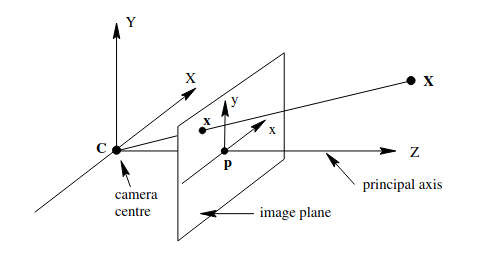
\includegraphics[scale=1]{images/camera_model/pinhole_visualisation.png}
    \caption{Модель стенопа. C --- центральная точка, p --- главная точка.}
~\label{fig:pinhole_model}
\end{figure}

\begin{figure}[h!]
        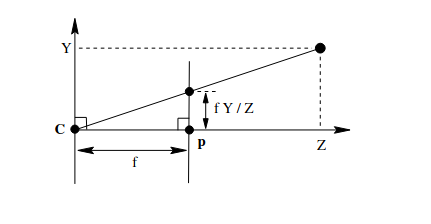
\includegraphics[scale=1]{images/camera_model/pinhole_visualisation_side.png}
        \caption{Модель в проекции на плоскость YZ. f --- фокусное расстояние.}
~\label{fig:pinhole_geometry}
\end{figure}

При использовании данной модели, точка $\overline{P} = (X_p, Y_p, Z_p)$ в
системе координат $C_{XYZ}$ проецируется на плоскость изображения по уравнению
~\eqref{eqn:pinhole_projection}, описанному в~\cite{multiview_cv}.

\begin{equation}
    \overline{A} = (X_A, Y_A, Z_A) \rightarrow (fX_A/Z_a, fY_A/Z_A) = \overline{a} 
~\label{eqn:pinhole_projection}
\end{equation}.

Уравнение \eqref{eqn:pinhole_projection} проецирует вектор из $\mathbb{R}^3$ в
пространство $\mathbb{R}^2$. Подобное преобразование можно выписать в матричной
форме через однородные преобразования, как это было сделано в
~\cite{multiview_cv}.
\begin{equation}
    \begin{pmatrix}
        f X_A \\
        f Y_A \\
        Z_A
    \end{pmatrix} = 
    \begin{bmatrix}
        f & 0 & 0 & 0 \\
        0 & f & 0 & 0 \\
        0 & 0 & 1 & 0
    \end{bmatrix} \begin{pmatrix}
        X_A\\
        Y_A\\
        Z_A\\
        1
    \end{pmatrix}
~\label{eqn:pinhole_matrix_projection_ideal}
\end{equation}

\par

Уравнение \eqref{eqn:pinhole_matrix_projection_ideal} описывает проецирование из
СК $C_{XYZ}$ на плоскость изображения.  Однако, уравнение
~\eqref{eqn:pinhole_matrix_projection_ideal} предполагает, что главная точка $p$
совпадает с центром системы координат плоскости изображения, что, в силу
неидеальности реальных камер, не всегда является правдой. Тогда уравнение
~\eqref{eqn:pinhole_matrix_projection_ideal} стоит переписать, чтобы оно
учитывало смещение главной точки относительно центра СК $xy$ плоскости
изображения:
    
\begin{equation}
    \overline{a} = \begin{pmatrix}
        fX_A + Z_A p_x\\
        fY_A + Z_A p_y\\
        Z_A
    \end{pmatrix} = \begin{bmatrix}
        f & 0 & p_x & 0 \\
        0 & f & p_y & 0 \\
        0 & 0 & 1 & 0
    \end{bmatrix} \begin{pmatrix}
        X_A\\
        Y_A\\
        Z_A\\
        1
    \end{pmatrix}
~\label{eqn:pinhole_matrix_projection_real}
\end{equation}

Выпишем матрицу проекции из уравнения ~\eqref{eqn:pinhole_matrix_projection_real}:
\begin{equation}
    K = \begin{bmatrix}
        f & 0 & p_x\\
        0 & f & p_y\\
        0 & 0 & 1
    \end{bmatrix}
\end{equation}

Эта матрица в~\cite{multiview_cv} называется матрицей калибровки, однако в своей
работе я буду называть ее матрицей камеры. 

Помимо этого, нужно иметь модель искажений камеры.
В своей работе я буду использовать модель искажений, описанную в
~\cite{opencv_calibration_tutorial} так как она является ''стандартной'' для этой
библиотеки.  Не буду вдаваться в подробности так как я использовал обычные
камеры, а зачастую, даже на обычных потребительских камерах, коэффициенты
искажений хоть и не являются нулевыми, довольно малы.

\subsection{Реализация калибровки внутренних параметров}
\label{sec:camera_intrinsics_calibration}
Калибровка внутренних параметров использует доску ChArUco для расчета матрицы
камеры и коэффициентов искажения. В файле
\texttt{calibration/intrinsics\_calibration.py} имплементирует алгоритм, очень
похожий на описанный в\cite{opencv_calibration_tutorial}, но с небольшими
изменениями.



Сначала я сформулировал более точное техническое задание для программы калибровки внутренних параметров. 
Эта программа должна:
\begin{enumerate}
  \item получить на вход ряд параметров,
  \item создать объект видеозахвата на основе этих парамеров,
  \item создать объект, отображающий параметры доски ChArUco, на основе этих парамеров,
  \item снимать видео с ChArUco доской, пока пользователь не введет команду прекращения съемки,
  \item после завершения съемок калибрует камеру при помощи \texttt{cv2.calibrateCamera},
  \item после калибровки, сохраняет внутренние данные в виде pkl-файла, содержащего в себе объект \texttt{dict}.
\end{enumerate}

\begin{figure}[h!]
  \begin{center}
    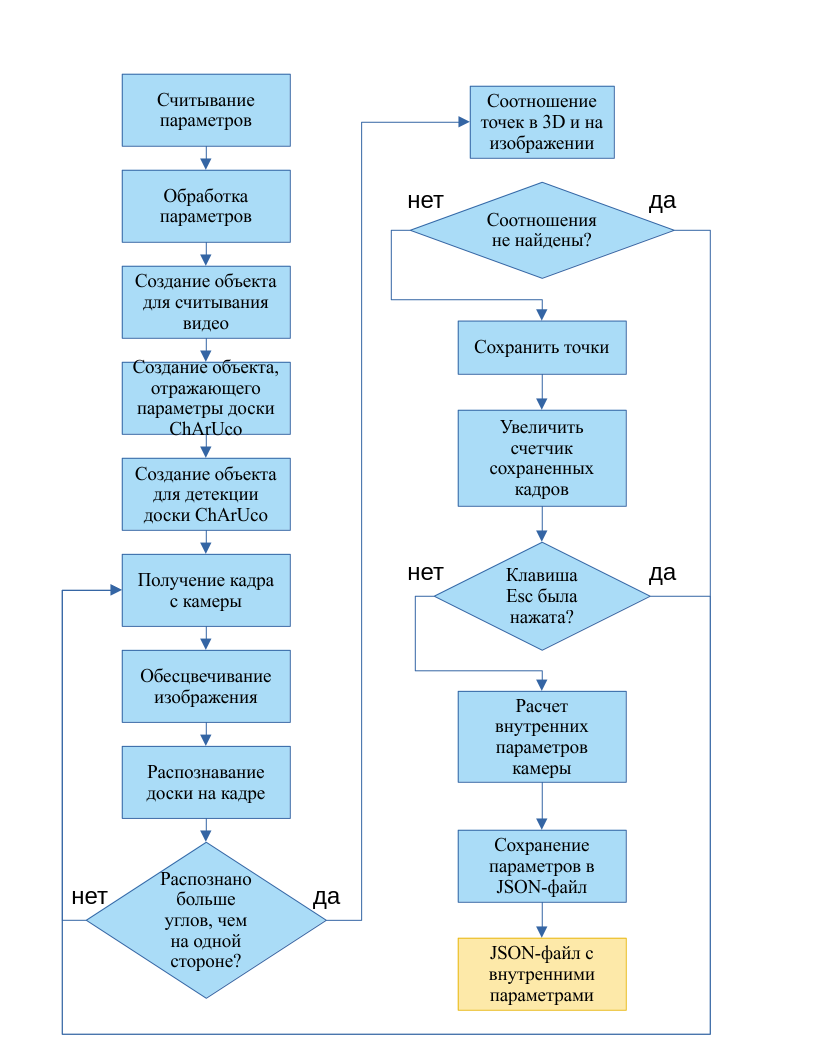
\includegraphics[width=0.95\textwidth]{images/block-schemes/intrinsics_scheme.png}
  \end{center}
  \caption{Блок-схема алгоритма калибровки камер}
  \label{fig:intrinsincs_block_scheme}
\end{figure}

Блок-схема алгоритма калибровки внутренних параметров камеры изображена на
рисунке \ref{fig:intrinsincs_block_scheme}.

Параметры нужны для того, чтобы с каждой из исполняемых програм было удобнее работать.
В каждой из них есть ряд параметров, которые можно указать при запуске. 
Они позволяют отлаживать код быстрее, а также позволяют выбирать нужные файлы,
камеры и другие вещи, которые могут меняться, "на ходу".
\par
\texttt{cam\_id} --- этот аргумент указывает идентификационный номер камеры.
На основании этого аргумента откроется устройство захвата через
\texttt{cv2.VideoCapture}. 
\listingsection{
../calibration/intrinsics_calibration.py
}{CAMID}

Также, есть два аргумента влияющих на формат названия:
\begin{itemize}
  \item \texttt{--no-error-name} --- если этот аргумент использован, то в
    названии выходного файла не будет указано значение ошибки перепроекции,
  \item \texttt{--no-frames-name} --- если этот аргумент использован, то в
    назыании выходного файла не будет указано количество записанных кадров для
    калибровки.
\end{itemize}
\listingsection{
../calibration/intrinsics_calibration.py
}{NAMEARGS}

Параметр \texttt{--output} хранит путь к выходному файлу и основу для его
названия, то есть, если этот аргумент имеет значение \texttt{calibration\_results/calibration\_L},
то в итоге выходной файл будет лежать в директории
\texttt{calibration\_results} и иметь название, например, \\
\texttt{calibration\_L\_frames=623\_error=1.5265531081871597.pkl}.
\listingsection{
../calibration/intrinsics_calibration.py
}{OUTPUTNAME}

Параметр \texttt{--capture\_json} хранит путь к файлу с параметрами создания
объекта захвата. Этот параметр нужен чтобы открывать объекты с одинаковыми
параметрами каждый раз.
\listingsection{
../calibration/intrinsics_calibration.py
}{CAPTUREJSON}

Параметр \texttt{--num-threads} указывает сколько потоков может использовать
OpenCV для проведения расчетов.
\listingsection{
../calibration/intrinsics_calibration.py
}{NUMTHREADS}

После введения аргументов, происходит их разбор и сохранение id камеры в
отдельную переменную:
\listingsection{
../calibration/intrinsics_calibration.py
}{PARSE}

Создается объект, отображающий параметры доски. Это нужно для того, чтобы
камера калибровалась на основе рельных известный расстояний. После этого, на основе
созданной доски, создается объект \texttt{cv2.aruco.CharucoDetector}, который
нужен для правильного распознаваия доски на изображении:
\listingsection{
../calibration/intrinsics_calibration.py
}{CREATECHARUCO}

Инициализируются переменные, необходимые для хранения точек, которые потребуются
для калибровки, также счетчик записанных кадров:
\listingsection{
../calibration/intrinsics_calibration.py
}{BASICINIT}

Открывается объект захвата, на основе заданных id камеры и файла конфигурации.
Функция \texttt{create\_caupture\_from\_json} определена в разделе с
вспомогательными функциями.
\listingsection{
../calibration/intrinsics_calibration.py
}{CREATECAPTURE}

После чего, начинается цикл захвата изображений, который идет до тех пор, пока
пользователь не нажмет на кнопку Escape.Последующий код будет
находиться внутри цикла \texttt{while True:}, пока я не укажу обратное.
\par
Сначала считывается изображение с объекта захвата и по переменной
\texttt{ret} проверяется, что изображение было успешно считано:
\listingsection{
../calibration/intrinsics_calibration.py
}{READFRAME}

После чего получается размер изображения, необходимый для калибровки:
\listingsection{
../calibration/intrinsics_calibration.py
}{GETSIZE}

Затем, изображение обесцвечивается, что необходимо для распознавания ChArUco доски:
\listingsection{
../calibration/intrinsics_calibration.py
}{DISCOLOR}

На grayscale-изображени распознается доска. Результатом работы этого кода
являются: 
\begin{itemize}
  \item набор углов клеток доски(\texttt{charuco\_corners})
  \item набор идентификаторов каждого из углов клеток(\texttt{charuco\_ids}),
  \item набор углов ArUco маркеров, расположенных на доске(\texttt{marker\_corners}),
  \item набор идентификаторов маркеров, расположенных на доске (\texttt{marker\_ids}).
\end{itemize}
После чего проверяется, был ли найден хотя бы один угол на доске.
В случае, когда не было найдено ни одного угла, исполнение программы
возвращается в начало цикла.
\listingsection{
../calibration/intrinsics_calibration.py
}{DETECT}

После этого, если углы и маркеры были обнаружены, они отрисовываются на
исходном изображении и результат обнаружения выводится на экран:
\listingsection{
../calibration/intrinsics_calibration.py
}{DISPLAY}

Далее проверяется, достаточно ли углов было найдено. 
Углов достаточно, когда их больше, чем максимальное возможное количество углов,
лежащих на одной прямой. Это условие гарантирует, что не все найденные углы
лежат на одной прямой. Если углов достаточно, то при помощи метода
\texttt{matchImagePoints} объекта доски \texttt{charuco\_board}, созданного
ранее, получаются:
\begin{itemize}
  \item координаты точек в пространстве --- \texttt{cur\_object\_points}, 
  \item координаты точек на изображении --- \texttt{cur\_image\_points}.
\end{itemize}
Эти переменные отображают соотвествие между координатами в трехмерном
пространстве и точками на изображении.
После чего, проверяется, получилось ли получить хотя бы одно соответствие между
точками. Если это условие выполняется, то счетчик сохраненных кадров
увеличивается на 1 и данные точки сохраняются для дальнейшей обработки. В
противном случае, исполнение возвращается в начало цикла.
\listingsection{
../calibration/intrinsics_calibration.py
}{SAVEPOINTS}

Далее, проверяется нажатие клавишы. Если была нажата клавиша Escape, то цикл прекращается.
\listingsection{
../calibration/intrinsics_calibration.py
}{WAITKEY}

На этом, считываение и обработка кадров заканчивается. Следующий код идет после цикла \texttt{while True}.

Как только пользователь нажал клавишу Escape, считываение кадров прекращается,
и закрываются все открытые для вывода изображений окна, а также освобождается
объект захвата \texttt{cap}.
\listingsection{
../calibration/intrinsics_calibration.py
}{CV2CLOSE}

Затем, вычисляются внутренние параметры камеры при помощи функции\\
\texttt{cv2.calibrateCamera}:

\listingsection{
../calibration/intrinsics_calibration.py
}{CALIBRATION}

Результатом работы этого кода являются:
\begin{itemize}
  \item \texttt{precision} --- дробное число, отражающее ошибку перепроекции с данными внутренними параметрами,
  \item \texttt{camera\_matrix} --- матрица камеры, о которой говорилось в \ref{sec:camera_model},
  \item \texttt{dist\_coeffs} --- коэффициенты искажений камеры.
\end{itemize}

Как только камера была откалибрована, формируется словарь с полученными данными, формируется название, и записывается в .pkl файл.
\listingsection{
../calibration/intrinsics_calibration.py
}{SAVEDATA}

    

\subsection{Калибровка положения}

Было описано как происходит проецирование точек на плоскость камеры. Однако, в
реальности не всегда удобно считать камеру центром СК. Поэтому, часто вводится
некая глобальная система координат. Назовем ее $O_{X_0Y_0Z_0}$. Эта система
координат связана с системой координат $C_{XYZ}$ через однородное
преобразование $T_{CO}$. Допустим, что вектор $\overline{A}_C \in \mathbb{R}^4$
представляет собой однородные координаты точки $A$ в СК $C_{XYZ}$, а вектор
$\overline{A}_O \in \mathbb{R}^4$ представляет собой координаты этой же точки в
СК $O_{X_0Y_0Z_0}$. Тогда:

\begin{equation}
    \overline{A}_C = T_{CO} \cdot \overline{A}_O.
\label{eqn:basic_matrix_tf}
\end{equation}
Если учесть~\eqref{eqn:pinhole_matrix_projection_real} и
подставить~\eqref{eqn:basic_matrix_tf} в него, получится:

\begin{equation}
\begin{gathered}
    \overline{a} = K \cdot \overline{A_C} = \\
    = K \cdot T_{CO} \cdot \overline{A_O}
\end{gathered}
\label{eqn:full_projection}
\end{equation}
При этом, матрица однородного преобразования $T_CO$ состоит из двух частей:
\begin{equation}
\begin{gathered}
    T_CO = \left[ R \quad \vline \quad t \right] = \\
    = \left[
        \qquad R \qquad \vline \begin{pmatrix}
        x_t\\
        y_t\\
        z_t
    \end{pmatrix}
    \right]
\end{gathered}
\label{eqn:projection_matrix_tf}
\end{equation}
$t$ --- вектор смещения, являющийся, по сути, просто положением доски, а $R$ ---
матрица поворота, полученная по формуле Родрига~\cite{opencv_rodrigues}:
\begin{equation}
\begin{gathered}
    R = \cos(\theta) I + (1 - \cos(\theta))r r^T + \sin(\theta) \begin{bmatrix}
         0   & -r_z & r_y\\
        r_z  & 0    & -r_x\\
        -r_y & r_x  & 0
    \end{bmatrix}
\end{gathered}
\label{eqn:rodrigues_formula}
\end{equation}
При этом, вектор поворота $r$ является трехмерным вектором, норма которого равна
$\theta$ --- углу поворота, а нормированные значения --- ось поворота.

\par
Собирая вместе уравнения \eqref{eqn:rodrigues_formula}, \eqref{eqn:projection_matrix_tf}, \eqref{eqn:full_projection}, получим:
\begin{equation}
\begin{gathered}
    \overline{a} = K \cdot \left[R \quad \vline \quad t\right] \cdot \overline{A}_O = \\
    = P \cdot \overline{A}_O
\end{gathered}
\label{eqn:proj_fomula_with_projection_matrix}
\end{equation}
Здесь $P$ --- матрица проекции. У каждой камеры есть своя матрица проекции, через которую можно определить как точка в пространстве будет спроецирована на плоскость изображения.
Рассмотрим каждую составляющую, чтобы понять от чего зависит матрица проекции:
\begin{itemize}
    \item $K$ --- матрица внутренних характеристик, полученная в
    \ref{sec:camera_intrinsics_calibration}, она известна для камеры и не
    меняется для камеры, к которой относится,

    \item $R$ --- матрица поворота, при этом, эта матрица имеет лишь три
    независимых параметра, что видно из \ref{eqn:rodrigues_formula},

    \item $t$ --- вектор смещения.
\end{itemize}
\par
Для калибровки положения необходимо найти матрицу проекции для каждой из
используемых камер. То есть нужно найти всего 6 неизвестных параметров. В OpenCV
это происходит при помощи ChArUco доски. На этой доске есть ряд характерных
точек, при этом, зная размер доски, легко расчитать расстояния между этими
точками. Таким образом, у нас есть относительные положения точек. Нам известны
их положения $\overline{A}_O$ и также нам известны их проекции на камере
$\overline{a}$. Нужно теперь подобрать такие значения $r$ и $t$, чтобы ошибка
перепроецирования $\overline{A}_O \rightarrow \overline{a}$ была минимальной.
Это делается методом наименьших квадратов в~\cite{opencv_charuco_pose}. Эту функцию
я использую в программе \texttt{calibration/orientation\_calibration.py} чтобы
получить положения доски ChArUco относительно камер. После чего, достаточно найти обратную к $T_{CO}$ матрицу, чтобы получить положение камер относительно центра $O$ системы координат $O_{X_0Y_0Z_0}$.

\subsection{Реализация калибровки положения}
Данная программа должна выполнять следующие вещи:
\begin{itemize}
  \item Открывать один или несколько источников видео,
  \item загружать внутренние параметры используемых камер,
  \item создать объекты параметров доски и детектора параметров,
  \item считывать кадр с каждого из открытых источников,
  \item распознавать доску ChArUco на кадрах,
  \item оценивать положение и поворот доски относительно камеры,
  \item сохранять положение доски в .pkl файл со словарем, содержащим данные о
    положении для каждой из указанных камер.
\end{itemize}

Блок схема данной программы изображена на рисунке \ref{fig:orientation_calibration_scheme}

\begin{figure}[h!]
  \begin{center}
    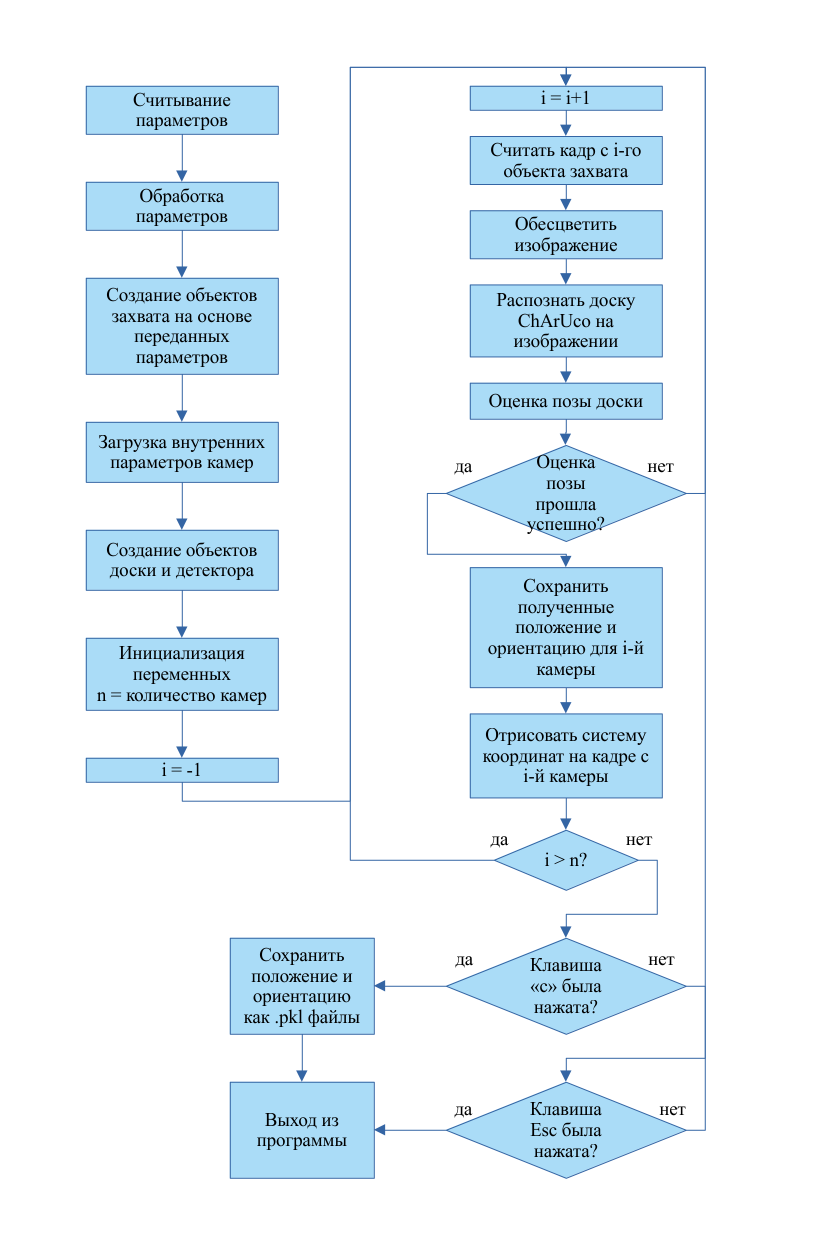
\includegraphics[width=0.95\textwidth]{images/block-schemes/orientation_scheme.png}
  \end{center}
  \caption{Блок-схема алгоритма калибровки положения камер.}\label{fig:orientation_calibration_scheme}
\end{figure}

Калибровка положения реализована в файле \texttt{orientation\_calibration.py}.

У этой программы, как почти у любой другой в этом проекте, есть ряд аргументов
при запуске из коммандной строки. Перед тем, как программа начнет исполнение
алгоритма калибровки положения, в ней вводятся параметры, описанные дальше.

Параметр \texttt{input\_sources} хранит в себе видео или камеры, по которым
будет производиться калибровка.
\listingsection{
../calibration/orientation_calibration.py
}{INPUT_SOURCES}

Параметр \texttt{--intrinsics-files} хранит в себе пути к файлам с внутренними
параметрами камеры, которые были получены на предыдущем этапе калибровки.
\listingsection{
../calibration/orientation_calibration.py
}{INTRINSICS_FILES}

Параметр \texttt{--output} хранит путь где будут сохранены выходные файлы, а
так же префикс, с которого будут начинаться их названия.
\listingsection{
../calibration/orientation_calibration.py
}{OUTNAME}

Параметр \texttt{--separate} является флагом, если он использован, то данные
калибровки положения будут сохранены как два разных файла, в противном
случае, данные для двух камер будут сохранены в один файл.
\listingsection{
../calibration/orientation_calibration.py
}{SEPARATE}

Параметр \texttt{--display-scale} хранит в себе значение масштаба выводимых
изображений.
\listingsection{
../calibration/orientation_calibration.py
}{DISPLAY_SCALE}

После введения параметров проводится их разбор, сохранение списка источников
видео и масштаба, установка количества потоков и проверка наличия всех файлов
внутренних параметров.
\listingsection{
../calibration/orientation_calibration.py
}{INIT}

После чего:
\begin{itemize}
  \item проверяется, все ли переданные источники состоят из цифр, что означает, что они являются камерами,
  \item создается список, где будут храниться объекты захвата видео,
  \item на основе параметров либо открываются источники, не являющиеся
    камерами, либо открываются камеры через
    \texttt{create\_capture\_from\_json},
  \item созданные объекты захвата добавляются в созданный список.
\end{itemize}
\listingsection{
../calibration/orientation_calibration.py
}{PREP_CAMS}

Для корректной оценки положения камер, нужно загрузить их внутренные параметры.
Для этого, открывается каждый из указанных .pkl файлов, из словаря,
находящегося в нем, берутся матрица камеры и коэффициенты искажения.
\listingsection{
  ../calibration/orientation_calibration.py
}{LOAD_INTR}

Для детекции ChArUco доски, нужно создать объекты доски и детектора.
\listingsection{
  ../calibration/orientation_calibration.py
}{CHARUCO_SETUP}

После чего, проводится инициализация перед началом считывания. В ней
создаются: флаг успешного считывания, список полученных векторов поворота,
список полученных векторов положения и список внешних характеристик.
\listingsection{
  ../calibration/orientation_calibration.py
}{READ_INIT}

Затем, пока пользователь не даст комманду и пока считывание проходит
успешно, из каждого из созданных устройств захвата считывается кадр. Все
дальнейшие листинги кода происходят внутри цикла \texttt{while all\_ok:}, пока не
будет сказано обратное.
\listingsection{
  ../calibration/orientation_calibration.py
}{READ_FRAME}

Для корректной детекции доски, изображение нужно обесцветить.
\listingsection{
  ../calibration/orientation_calibration.py
}{DISCOLOR}

На обесцвеченном изображении созданный ранее детектор распознает доску и
возвращает найденные углы клеток доски, номера углов клеток, углы маркеров
на доске, номера маркеров.
\listingsection{
  ../calibration/orientation_calibration.py
}{DETECT}

Теперь при помощи функции \texttt{estimatePoseCharucoBoard} из библиотеки
OpenCV производится оценка положения доски на изображении. Эта функция
возвращает:
\begin{itemize}
  \item \texttt{ret} --- Флаг успешной оценки позы,
  \item \texttt{rvec} --- вектор поворота, который можно преобразовать в
    матрицу поворота при помощи формулы Родрига.
  \item \texttt{tvec} --- вектор смещения.
\end{itemize}
\listingsection{
  ../calibration/orientation_calibration.py
}{POSE_ESTIM}

Чтобы пользователь мог увидеть где находится центр координат, полученные
выше оси отрисовываются на изображении с камеры.
\listingsection{
  ../calibration/orientation_calibration.py
}{POSE_DISPLAY}

После чего, считывается клавиша с клавиатуры, чтобы пользователь мог
прекратить считываение кадров и сохранить данные, или прервать исполнение
программы.
\listingsection{
  ../calibration/orientation_calibration.py
}{CMD_INPUT}
Функция \texttt{save}:
\listingsection{
  ../calibration/orientation_calibration.py
}{SAVE_FUNC}

\section{Распознавание рук}
Нейросетевые методы распознавания не являются темой моей дипломной работы,
поэтому я не буду углубляться в то, как они работают, я буду использовать уже готовую модель для выделения ключевых точек руки.

Сформулируем, что должно быть в этом модуле:
\begin{itemize}
  \item Считываение кадров с источника видео,
  \item предобработка, например, перевод в цветовое пространство RGB,
  \item распознавание точек на руке,
  \item опциональная отрисовка результатов детекции,
  \item возврат результатов детекции как массив точек на изображении.
\end{itemize}

В модуле распознавания рук описан класс \texttt{CaptureDetector}, который
открывает выбранный источник видео и на каждом полученном кадре находит
ключевые точки и возвращает их в определенном формате. Использование такой
структуры позволяет создать два отдельных объекта разпознавания для рук.
Благодаря этому, распознавание для каждой камеры может происходить параллельно, или, например, во время отладки, можно запустить детекцию руки только для одной камеры.

Для распознавания руки я решил использовать MediaPipe API от Google. Этот
программный интерфейс является довольно простым в работе и есть для языка
Python, который я использую.
MediaPipe имеет несколько режимов распознавания:
\begin{enumerate}
  \item на статичной картине --- \texttt{mp.tasks.vision.RunningMode.IMAGE},
  \item на декодированном видео --- \texttt{mp.tasks.vision.RunningMode.VIDEO},
  \item на потоке видео, в ``прямом эфире'' --- \texttt{mp.tasks.vision.RunningMode.LIVE\_STREAM}.
\end{enumerate}

Изначально, я предполгалал, что третий режим подойдет лучше всего, однако из-за
того, что документация на MediaPipe довольно ограничена и почти не описывает
этот режим, я решил использовать значительно лучше задокументированный режим
\texttt{VIDEO}. Этот режим распознает руку на каждом статичном изображении, как
и \texttt{IMAGE}, но, в отличие от него, в нем также используется отслеживание
движений между кадрами, что позволяет улучшить качество предсказаний модели.

\subsection{Класс \texttt{CaptureDetector}}
Распознавание рук происходит в классе \texttt{CaptureDetector}, описанном в файле \\ 
\texttt{detection/capture\_detector.py}
Этот класс используется как абстракция для выделения руки на изображении. У
этого класса есть две главные функции:
\begin{itemize}
  \item \texttt{\_\_init\_\_} --- инициализация,
  \item \texttt{process\_one\_frame} --- функция получения и обработки кадра.
\end{itemize}

\subsubsection{Инициализация \texttt{\_\_init\_\_()}}
Класс \texttt{CaptureDetector} при инициализации принимает на вход два аргумента:
\begin{itemize}
  \item \texttt{capture} --- уже созданный объект захвата
    \texttt{cv2.VideoCapture} для видео. Этот объект будет использоваться для
    получения кадров с камеры.
  \item \texttt{model\_path} --- путь к весам модели для распознавания.
\end{itemize}

В начале иницализации, переданный объект захвата сохраняется в поле класса
\texttt{cap}, а также из объекта захвата извлекаются ширина и высота изображения.
\listingsection{
  ../detection/capture_detector.py
}{INIT_CAP}

После этого создается переменная \texttt{base\_options}, хранящая в себе
базовые параметры программного интерфейса, а в частности параметры модели.
Создается объект \\\texttt{hand\_landmarker\_options}. Эта переменная нужна
только для того, чтобы строка с созданием объекта параметров детектора не была слишком
длинной. Для этого же создается переменная \texttt{running\_mode}.
Затем, создается поле \texttt{options}, которое хранит объект класса 
\\\texttt{ mp.tasks.vision.HandLandmarkerOptions}. Это поле отражает следующие
параметры распознавания:
\begin{itemize}
  \item путь к весам модели,
  \item режим распознавания,
  \item количество рук, которые модель может распознать на одном кадре.
\end{itemize}
После чего, наконец, создается сам объект детектора на основе введенных ранее
параметров и записывается в поле \texttt{landmarker}.
\listingsection{
  ../detection/capture_detector.py
}{INIT_TASK}
На этом заканчивается инициализация объекта \texttt{CaptureDetector}.

\subsubsection{Обработка изображения \texttt{process\_one\_frame}}
Для того, чтобы считать один кадр с объекта захвата и распознать ключевые
точки на нем, используется функция
\texttt{process\_one\_frame}.
Эта функция принимает на вход один аргумент --- \texttt{return\_frame}. Если
этот аргумент имеет истинное значение, то эта функция вместо кадра вернет
\texttt{None}.

В начале этой функции происходит 
\begin{enumerate}
  \item считывание изображения;
  \item проверка того, что изображение было считано;
  \item перевод из стандартного для OpenCV цветого пространства BGR в RGB,
    необходимое для корректного распознавания точек руки;
  \item создание объекта изображения \texttt{mediapipe.Image}, который
    используется в программном интерфейсе для распознавания.
\end{enumerate}
\listingsection{
  ../detection/capture_detector.py
}{FRAME_PREPROCESS}

Также, для улучшения распознавания, нужно знать время, в которое был считан кадр,
для чего используется метод \texttt{get} класса \texttt{VideoCapture}.
\listingsection{
  ../detection/capture_detector.py
}{GET_TIME}

После чего, с учетом временной метки кадра, получается результат детекции,
который, нужно заметить, является объектом класса \texttt{HandLandmarkerResult} 
из библиотеки MediaPipe.
\listingsection{
  ../detection/capture_detector.py
}{GET_DETECTION}

Затем, если функция должна вернуть кадр вместе с массивом распознанных точек,
то кадр переводится обратно в цветовое пространство BGR, необходимое для
корректного отображения изображения. Если же функция не должна возвращать
кадр, то его "указатель" обнуляется.
\listingsection{
  ../detection/capture_detector.py
}{FRAME_CONVERSION}

Также, перед тем как вытаскивать элементы из объекта результата детекции,
нужно проверить, было ли обнаужено хоть что-нибудь.
\listingsection{
  ../detection/capture_detector.py
}{DETECTION_CHECK}

В конце функции 
\begin{itemize}
  \item Выбирается результат для первой руки в списке распознанных рук,
  \item из результата детекции вытаскиваются координаты распознанных точек,
  \item полученные точки преобразуются из относительных координат на отрезке
    $\left[0; 1\right]$ в абсолютные координаты, измеряемые в пикселях,
  \item полученный список точек возвращается вместе с кадром.
\end{itemize}
\listingsection{
  ../detection/capture_detector.py
}{RESULT_PREPARATION}

В деструкторе класса закрывается модель для детекции, а также освобождаются объекты захвата.
\listingsection{
  ../detection/capture_detector.py
}{DESTRUCTOR}

\subsection{Пример запуска}
Пример того, как используется класс \texttt{CaptureDetector} написан в файле\\
\texttt{detection/run\_detection.py}.

\section{Теория для позиционирования}

В рамках своей работы, я делаю систему, которая на основе данных с камер распознает положение рук. Одним из методов получения координат точки на основании ее проекций является триангуляция.
\subsection{Постановка проблемы}
В \ref{sec:camera_model} была описана проекция на плоскость камеры. Очевидно,
что при этом происходит преобразование $\mathbb{R}^4 \rightarrow \mathbb{R}^3$,
то есть у нас теряется одна переменная. То есть для одной камеры получается система линейных уравнений:
\begin{equation}
    \begin{pmatrix}
        x_a\\
        y_a\\
        z_a
    \end{pmatrix} = \begin{pmatrix}
        f X_A + Z p_x\\
        f Y_A + Z p_y\\
        Z_A 
    \end{pmatrix} = \underset{3 \times 4}{P} \begin{pmatrix}
        X_A\\
        Y_A\\
        Z_A\\
        1
    \end{pmatrix}
\label{eqn:triangle_problem}
\end{equation}
Для определения координат в трехмерном пространстве, нужно найти $X_A$, $Y_A$,
$Z_A$, и при этом система \eqref{eqn:triangle_problem} содержит в себе 3
уравнения. Однако, если посмотреть на
уравнение~\eqref{eqn:pinhole_matrix_projection_real}, то несложно заметить, что
последнее уравнение в этой системе является вырожденным:
\begin{equation*}
    Z_A = Z_A
% \label{eqn:useless_triangle}
\end{equation*}
\par
Таким образом, для одной камеры имеется система из двух уравнений с тремя
неизвестными. Простейшим решением данной проблемы является добавление еще одной
камеры. Это позволит решить систему. В \cite{multiview_cv} и \cite{dlt_temugeb} описана данная задача и ее решение. 
\subsection{Уравнения для одной камеры}
Система для $i$-й камеры выглядит так~\cite{multiview_cv, dlt_temugeb}:
\begin{equation}
    \overline{a}_i = \alpha P_i \overline{A}_O,
\label{eqn:general_dlt}
\end{equation}
где $\overline{a}_i$ --- вектор проекции точки $A$ на плоскость изображения $i$-й камеры, $P_i$ --- матрица проекции для $i$-й камеры, а $\overline{A}_O$ --- координаты точки $A$ в глобальной системе координат $O_{X_0Y_0Z_0}$, а $\alpha$ --- коэффициент, относящий длину вектора в правой части уравнения к пиксельным координатам на изображении.
\par
 Представим матрицу проекции как три четырехмерных вектора:
\begin{equation}
    P_i = \begin{bmatrix}
        \overline{p}_{i1}\\
        \overline{p}_{i2}\\
        \overline{p}_{i3}\\
    \end{bmatrix}
\end{equation}
Известно, что вектора в левой и правой частях уравнения параллельны, а значит,
их векторное произведение равно нулю.
\begin{equation}
    \begin{pmatrix}
        a_{xi}\\
        a_{yi}\\
        1
    \end{pmatrix} \times \begin{pmatrix}
        \overline{p}_{i1} \overline{A}_O\\
        \overline{p}_{i2} \overline{A}_O\\
        \overline{p}_{i3} \overline{A}_O
    \end{pmatrix} = \begin{pmatrix}
        a_{yi} \overline{p}_{i3} \overline{A}_O - \overline{p}_{i2} \overline{A}_O\\
        \overline{p}_{i1} \overline{A}_O - a_{xi} \overline{p}_{i3} \overline{A}_O\\
        a_{xi} \overline{p}_{i2} \overline{A}_O - a_{yi} \overline{p}_{i1} \overline{A}_O
    \end{pmatrix} = \begin{pmatrix}
        0\\
        0\\
        0
    \end{pmatrix}
\label{eqn:full_cross_product}
\end{equation}
Упростим уравнение~\ref{eqn:full_cross_product}:
\begin{equation}
    \begin{pmatrix}
        a_{xi}\\
        a_{yi}\\
        1
    \end{pmatrix} \times \begin{pmatrix}
        \overline{p}_{i1} \overline{A}_O\\
        \overline{p}_{i2} \overline{A}_O\\
        \overline{p}_{i3} \overline{A}_O
    \end{pmatrix} = \begin{pmatrix}
        a_{yi} \overline{p}_{i3} - \overline{p}_{i2} \\
        \overline{p}_{i1} - a_{xi} \overline{p}_{i3} \\
        a_{xi} \overline{p}_{i2} - a_{yi} \overline{p}_{i1}
    \end{pmatrix} \overline{A}_O = \begin{pmatrix}
        0\\
        0\\
        0
    \end{pmatrix}
\label{eqn:cross_product_one_camera}
\end{equation}
\par
\subsection{Уравнения для двух камер}
Уравнение~\ref{eqn:cross_product_one_camera} описывает векторное
произведение векторов для одной камеры, теперь добавим вторую камеру:
\begin{equation}
\begin{gathered}
    \begin{pmatrix}
        a_{y1} \overline{p}_{13} - \overline{p}_{12} \\
        \overline{p}_{11} - a_{x1} \overline{p}_{13} \\
        a_{x1} \overline{p}_{12} - a_{y1} \overline{p}_{11}
    \end{pmatrix} \overline{A}_O = \begin{pmatrix}
        0\\
        0\\
        0
    \end{pmatrix} \\
    \begin{pmatrix}
        a_{y2} \overline{p}_{23} - \overline{p}_{22} \\
        \overline{p}_{21} - a_{x2} \overline{p}_{23} \\
        a_{x2} \overline{p}_{22} - a_{y2} \overline{p}_{21}
    \end{pmatrix} \overline{A}_O = \begin{pmatrix}
        0\\
        0\\
        0
    \end{pmatrix} \\
\end{gathered}
\label{eqn:two_cameras_cross_separate}
\end{equation}
Совместим в одну систему:
\begin{equation}
    \begin{pmatrix}
        a_{y1} \overline{p}_{13} - \overline{p}_{12} \\
        \overline{p}_{11} - a_{x1} \overline{p}_{13} \\
        a_{x1} \overline{p}_{12} - a_{y1} \overline{p}_{11}
        a_{y2} \overline{p}_{23} - \overline{p}_{22} \\
        \overline{p}_{21} - a_{x2} \overline{p}_{23} \\
        a_{x2} \overline{p}_{22} - a_{y2} \overline{p}_{21}
    \end{pmatrix} \overline{A}_O = \begin{pmatrix}
        0\\
        0\\
        0
    \end{pmatrix}
\end{equation}
\subsection{Решение системы и минимизация шумов}
``В реальном мире могут быть шумы, тогда система принимает вид 
\begin{equation}
M \overline{A}_{O} = w
\label{eqn:noise_introduction}
\end{equation}
Нужно решить эту систему с минимальным шумом $w$''\cite{dlt_temugeb}. Сделать это позволяет
SVD-разложение матрицы $M$:
\begin{equation}
    M \overline{A}_O = U S V^T \overline{A}_O
\end{equation}
Чтобы прийти к минимальному шуму $w$, возьмем скалярное произведение левой и правой частей уравнения \eqref{eqn:noise_introduction}:
\begin{equation}
    w w^T =   \overline{A}_O^T V S U^T U S V^T \overline{A}_O
\end{equation}
С учетом ортогональности матрицы $U: U^T U = I$:
\begin{equation}
    w w^T = \overline{A}_O^T V S S V^T \overline{A}_O = 
    \overline{A}_O^T V S^2 V^T \overline{A}_O
\label{eqn:noise_squared_svd_simplify}
\end{equation}
\par
Если взять в расчет ортогональность матрицы $V$ из-за свойств SVD-разложения, то получим, что если умножить $i$-ю строку $v_i$ матрицы $V$ на транспонированную матрицу $V^T$, то получится единичный вектор, где единичный элемент стоит на $i$-й позиции:
\begin{equation}
\begin{gathered}
    v_i V^T = \begin{pmatrix}
        0 & \cdots & \underset{i-1}{0} & \underset{i}{1} & \underset{i+1}{0} & \cdots & 0
    \end{pmatrix} = e_i^T \\
    V v_i^T = \begin{pmatrix}
        0 \\
        \vdots \\
        \underset{i-1}{0}\\
        \underset{i}{1}\\
        \underset{i+1}{0}\\
        \vdots\\
        0
    \end{pmatrix} = e_i
\end{gathered}
\end{equation}
Тогда, если мы возьем $\overline{A}_O$ в системе \eqref{eqn:noise_squared_svd_simplify} равным $i$-й строке матрицы $V$:
\begin{equation}
    w w^T = v_i^T V S^2 V^T v_i = s_i^2,
\end{equation}
где $s_i$ --- $i$-е сингулярное число в матрице $S$. Тогда достаточно взять $i$,
соответствующее минимальному сингулярному числу, в этом случае, квадрат 2-нормы
шума $w$ будет равен минимальному сингулярному числу.
Шум минимизирован.

\subsection{Улучшения}
В \cite{multiview_cv} описано несколько способов уменьшения шумов, если руки дойдут, я реализую что-то из них.

\section{Приведение руки к захвату манипулятора}
Этот шаг не имеет какого-то определенного подхода выписанного где-либо. Я для себя выделил три возможных метода приведения рук:
\begin{enumerate}
    \item Простой метод, основанный на большом и указательном пальцах,
    \item эвристический метод, включающий в себя ряд возможных способов взять объект,
    \item нейросетевой подход.
\end{enumerate}

\subsection{Простой метод}
\label{sec:gripper_basic_method}
\subsubsection{Описание метода}
Этот метод предполагает, что человек, использующий систему, берет все предметы
используя лишь указательный и большой палец. Для реализации данного метода
достаточно:
\begin{itemize}
    \item взять точки, принадлежащие большому и указательному пальцам,
    \item провести через эти точки две кривые, принадлежащие выбранным пальцам,
    \item найти кратчайший общий перпендикуляр между этими кривыми.
\end{itemize}
Простая визуализация этого метода изображена на рисунке \ref{fig:basic_gripping_simple_model}.
\begin{figure}[h!]
    \centering
    \includegraphics[width=0.5\textwidth]{example-image}
    \caption{Визуализация точки захвата}
~\label{fig:basic_gripping_simple_model}
\end{figure}
Точка захвата предмета будет лежать приблизительно по центру этого перпендикуляра.
\subsubsection{Преимущества и недостатки}
Главным преимуществом данного метода является простота и высокая надежность в тех случаях, где человек берет предмет подобным образом.
Главным недостатком является то, что этот метод крайне ограничен.

\subsection{Эвристический метод}
\subsubsection{Описание метода}
Этот метод заключается в том, чтобы выделить несколько распространенных способов
взятия объектов человеком, например, изображенных на рисунке
~\ref{fig:heuristic_gripping_variants}, после чего сделать функцию, которая
принимает на вход точки руки и оценивает к какому виду захвата объекта текущая
конфигурация точек ближе всего.

\begin{figure}
    \includegraphics[width=.3\textwidth]{example-image}\hfill
    \includegraphics[width=.3\textwidth]{example-image}\hfill
    \includegraphics[width=.3\textwidth]{example-image}
    \\[\smallskipamount]
    \includegraphics[width=.3\textwidth]{example-image}\hfill
    \includegraphics[width=.3\textwidth]{example-image}\hfill
    \includegraphics[width=.3\textwidth]{example-image}
    \caption{Способы захвата}
\label{fig:heuristic_gripping_variants}
\end{figure}

\subsubsection{Преимущества и недостатки}
Главным преимуществом является некоторое по сравнению с простым методом, также в
отличие от нейросетевых методов, описанных дальше, этот метод требует
значительно меньше человекочасов для реализации.
\par
Главным недостатком является то, что этот метод, будучи основанным на выведенной
человеком эвристике, может оказаться неточным и часто путать способы захвата.
Также, из-за выделения характеристик каждого захвата человеком, могут быть упущены детали, что также понизит его точность.

\subsection{Нейросетевой метод}
\subsubsection{Описание метода}
Этот метод близок к эвристическому, но основан на том, чтобы натренировать
модель, которая по входному массиву точек будет определять точку схвата. Для
тренировки модели, однако, нужен большой размеченный датасет, где на каждой
конфигурации точек отмечена точка захвата.

\subsubsection{Преимущества и недостатки}
Преимуществом данного метода перед остальными является потенциально высокая точность и универсальность, при достаточно большом и качественном датасете.
\par
Недостатком, же, является значительные требования по времени и ресурсам. Время
нужно чтобы собрать и разметить датасет для обучения, ресурсы в виде видеокарт
нужны для обучения. Ни того, ни другого у меня пока что нет.
 
\section{Выбор инструментов}
На основе списка поставленных задач и описанной теории, необходимой для их реализации, я выбрал набор инструментов, при помощи которых я буду реализовывать систему, описанную ранее.

\subsection{Выбор языка}
Для этой работы стоял выбор между двумя языками: C++ и Python. 
\par
C++ хорош своим быстродействием, а также обширным набором библиотек.
Помимо этого, есть ряд преимуществ, которые больше связаны с личными предпочтениями.
Однако, C++ имеет один ключевой для этой работы недостаток. По моим и не только
моим наблюдениям, реализация одного и того же программного продукта на C++
займет значительно большее время, чем реализация этого же программного продукта
на Python.
\par
Среди преимуществ Python можно выделить простоту использования, а также высокую читаемость кода. Как было сказано выше, программы на Python пишутся быстрее и проще, чем на C++. Однако из недостатков Python имеет крайне малую скорость работы, отсутствие указателей, отсутствие строгой типизации, полностью динамическую типизацию и ряд других вещей. Так или иначе, Python гораздо лучше подходит для прототипирования, чем C++, а в своей работе, я делаю скорее прототип, нежели полноценный продук, я буду использовать Python.

\subsection{Работа с видео}
Для работы с видео и изображениями и их обработки отлично подходит библиотека
OpenCV, доступная для C++ и Python. У меня есть опыт работы с ней, к тому же она
широко известна, хорошо задокументирована и постоянно обновляется.

\subsection{Параметры камеры}
Для калибровки камер сущетсвует хорошо
задокументированные\cite{opencv_calibration_tutorial, opencv_charuco_pose}
методы в OpenCV, которые позволяют без особых сложностей получить матрицу
камеры. Также, для определения матрицы проекции понадобится какой-то инструмент
для работы с матрицами и поворотами. Для этого я буду использовать классические
бибиотеки для Python: NumPy и SciPy. NumPy в первую очередь нужен для более
быстрой и удобной работы с массивами и матрицами так как предоставляет огромное
множество полезных методом. SciPy в своей работе я в основном использую для
работы с поворотами и их преобразованиями, так как SciPy реализует все эти
методы со множеством оптимизаций, лучше использовать их.

\subsection{Выделение ключевых точек руки}
Здесь не было обширного выбора, главное, что предлагалось в нескольких коротких
статьях, что я нашел --- MediaPipe от Google. Это библиотека для Python, которая
дает веса модели и API для взаимодействия с этой моделью для выделения ключевых
точек рук. В целом, эта библиотека имеет ряд неплохих примеров использования и
документацию. Примеры были очень полезны.
\par
Также, чуть позже, уже после того, как был реализован модуль детекции, я нашел альтернативу --- OpenPose. Однако применять ее времени уже нет.

\subsection{Триангуляция}
Так как по своей сути триангуляция является просто работой с матрицами, то все, что для нее потребуется --- это библиотеки NumPy и SciPy. Как ранее сказано, NumPy нужен для работы с матрицами, SciPy --- для работы с поворотами.

\subsection{Визуализация}
Чтобы реализация была как можно проще и имела как можно меньше ``странных''
зависимостей, для визуализации я буду использовать библиотеку matplotlib для
Python, которая позволяет строить графики в трехмерном пространстве. Точки я
буду визуализировать через нее.

\section{Разбор написанного кода}

\subsubsection{Предобработка изображения}
\subsubsection{Разпознавание при помощи MediaPipe}
\subsubsection{Формат найденных точек}

\subsection{Триангуляция}

\subsection{Преобразование к захвату манипулятора}

\subsection{Утилиты}
\subsubsection{Утилиты отрисовки}
\subsubsection{Утилиты для работы с файлами}
\subsubsection{Класс \texttt{Visualizer3D}}

\section{Замеры по точности}


\section{Заключение}

\subsection{Что работает}
\subsection{Что не работает}
\subsection{Модификации и усовершенствования}
\subsection{Ошибки при реализации}

\section{Приложения}

\section{Калибровка}
\subsection{Калибровка внутренних параметров}
\lstinputlisting[
    label=lst:intr_calib,
    caption={\texttt{intrinsics\_calibration.py}},
    language=python
    ]{../calibration/intrinsics_calibration.py}


\subsection{Калибровка положения}
\lstinputlisting[
    label=lst:pos_calib,
    caption={\texttt{orientation\_calibration.py}},
    language=python
    ]{../calibration/orientation_calibration.py} 

\section{Распознавание рук}
\subsection{Класс \texttt{CaptureDetector}}
\lstinputlisting[
    label=lst:capture_detector,
    caption={capture\_detector.py},
    language=Python
    ]{../detection/capture_detector.py}
\subsection{Программа для запуска детекции}
\lstinputlisting[language=Python]{../detection/run_detection.py}

\section{Триангуляция}
\subsection{Класс \texttt{Triangulator}}
\lstinputlisting[language=Python]{../positioning/triangulator.py}

\subsection{Файл для запуска определения положения руки}
\lstinputlisting[language=Python]{../positioning/run_hand_positioning.py}

\section{Приведение к захвату манипулятора}
\subsection{Тестовый способ}
\lstinputlisting[language=Python]{../gripper_conversion/gripper_converter.py}

\section{Утилиты}

\subsection{Класс \texttt{Visualizer3D}}
\lstinputlisting[language=Python]{../utils/visualizer_3d.py}

\subsection{Утилиты для работы с файлами}
\lstinputlisting[language=Python]{../utils/file_utils.py}

\printbibliography
% \bibliographystyle{plain}
% \bibliography{sources}
  
\end{document}
